%!TEX root = ../../thesis.tex
\define{\chapterpath}{\allchapterspath/relatedwork}
\define{\imgpath}{\chapterpath/img}

\chapter{Related Work}
\label{chapter:relatedwork}
\minitoc


In most robot social learning experiments today, there is a strong decoupling between the process of extracting useful informations from the interaction and the process of learning a new skill from these informations. For example, the human demonstrations were provided in a batch perspective where data acquisition is done before the learning phase. The properties of teaching interactions with a human in the loop was not yet considered in depth.

In this chapter we highlight the difference between systems learning from well controlled interactions and systems trying to close the interaction loop allowing more flexibility in the interaction process. These issues have began to be addressed in a subfield called \emph{interactive learning}  which combine ideas of social learning with extrinsic and intrinsic motivated learning. With this approach, the robot acquires a form of autonomy with respect to how to deal with the human in the loop. 

After presenting the related work in interactive learning, we broaden the scope of this work by linking with the computational modeling of language, some aspects of unsupervised learning, and specific works on ad-hoc team whose stated challenge is to enable cooperation without coordination in multi-agent scenarios. Finally, we present related works from the brain computer interfaces (BCI) community.

%%%%%%%%%%%%%%%%%%%%%%%%%%%%%%%%%%%%%%%%%%%%%%
%%%%%%%%%%%%%%%%%%%%%%%%%%%%%%%%%%%%%%%%%%%%%%
%%%%%%%%%%%%%%%%%%%%%%%%%%%%%%%%%%%%%%%%%%%%%%
%%%%%%%%%%%%%%%%%%%%%%%%%%%%%%%%%%%%%%%%%%%%%%
%%%%%%%%%%%%%%%%%%%%%%%%%%%%%%%%%%%%%%%%%%%%%%
\section{Interactive Learning}

In this section, we present a number of works considering the human component into the learning loop. We call this area of research \emph{interactive learning} \cite{nicolescu2003natural,breazeal2004tutelage}. It aims at developing machines that can learn by practical interaction with the user.

% Most of the systems presented in the previous section have not considered in depth the properties of teaching interactions with a human in the loop. The demonstrations are provided in a batch perspective where data acquisition is done before the learning phase.

\emph{Interactive learning} combines ideas of social learning with extrinsic and intrinsic motivated learning. It differs from the works presented in introduction in the sense that both the human and the robot are simultaneously involved in the learning process \cite{kaplan2002robotic,nicolescu2003natural,breazeal2004tutelage,thomaz2008teachable}. Under this approach, the teacher interacts with the robot and provides extra feedback or guidance. But in addition, the robot can act to improve its learning efficiency or elicit specific responses from the teacher. Recent developments have considered: extra reinforcement signals \cite{thomaz2008teachable}, action requests \cite{macl09airl}, disambiguation among actions \cite{chernova09jair}, preferences among states \cite{Mason2011}, iterations between practice and user feedback sessions \cite{judah2010reinforcement} and choosing actions that maximize the user feedback \cite{knox2009interactively}.

We decided to split this related work in four categories. Firstly, we present works combining multiple sources of information, such combining demonstration and feedback. Secondly, we present some studies about the behavior of human teaching robots. Thirdly, we present work that try to model some aspects of the user behavior or of the protocol. Fourthly, we present some work were the robot is active, trying to learn faster from or about the interaction. Finally, we discuss and situate our work in this scope.

% Interactive learning \cite{nicolescu2003natural,breazeal2004tutelage} aims at developing systems that can learn by practical interaction with the user and finds applications in a wide range of fields such as human-robot interaction, tutoring systems or human-machine interfaces.
% This type of learning combines ideas of learning from demonstration \cite{argall09survey}, learning by exploration \cite{thrun1992efficient} and tutor feedback \cite{kaplan2002robotic}. Under this approach the human teacher interacts with the machine and provides extra feedback or guidance. 
% In addition, the device can act to improve its learning efficiency. Approaches have considered: extra reinforcement signals \cite{thomaz2008teachable}, action requests \cite{lopes2009active}, disambiguation among actions \cite{chernova09jair}, preferences among states \cite{Mason2011}, iterations between practice and user feedback sessions \cite{judah2010reinforcement}, and choosing actions that maximize the user feedback \cite{knox2009interactively}. 

\subsection{Combining multiple learning source}

Researchers in the domain have considered mixing different types of paradigms in order to improve the quality of the interaction and of the learning process. They considered:

\begin{itemize}

\item Mixing environmental rewards with human rewards \cite{knox2010combining,griffith2013policy,grave2013learning}. The main problem is to balance the influence of the environmental reward with the human generated reward.

\item Iterations between practice and user feedback sessions \cite{judah2010reinforcement}. The learner first practices the task a few times and learns from some environmental reward. Then a user can observe it practice session and classifier some policies or actions as good or bad. The learner update its policies given the reward from the environment and the user critiques. And the process repeats again.

\item Giving some demonstrations first, and having the robot practicing the skill under human supervision (feedback or guidance) \cite{nicolescu2003natural,pardowitz2007incremental}.

\item Mixing concrete instructions and rewards to balance human efforts with communication efficiency \cite{pilarski2012between}.
% between instruction and reward to balance human effort with communication efficiency. Assistive technology, it is rare that you can control all aspect of the technology at once, for example, many active hand prosthesis have several modes of operation, two finger grip or full hand grip for example, where then fine control should be apply within that mode. Learning the preference of the user in terms of switching time based the past experience on the interaction. If what the system is not good, then the user can manually change it back. 

\item Combining learning from demonstration and mixed initiative control \cite{grollman2007dogged}. Mixed initiative control is when the control can transition smoothly from the demonstrator control to the robot control. In \cite{grollman2007dogged} the authors used this method to teach different behaviors to a robot, such as mirroring the head position with the tail position, or to seek for a red ball using the same algorithm.

\item Combining transfer learning, learning from demonstration and reinforcement learning \cite{taylor2011integrating}.

\item Considering demonstrations of parts of trajectories only. In \cite{akgun12hri}, the users only demonstrate some keyframe position along the line of the trajectory. The robot can then autonomously infer a trajectory that math with each keyframe position.

\end{itemize}

But researchers also created new learning paradigms, such as learning from users' preferences \cite{Mason2011,akrour2011preference}. In this new paradigm, the system learns the preferences of the human and will pro-actively generalize and apply them autonomously. 

In \cite{Mason2011}, the user starts by teleoperating the robot and can mark some states as good or bad. From this data, the robot can create a user profile. Next the robot can select its own goal without the need for human teleoperation. Once desirable state of the world has been reached, the human as a possibility to classify the state as good or bad again. The robot can update its user profile, and the process iterates.

% We have developed a robotic system that interacts with the user, and through repeated interactions, adapts to the user so that the system becomes semiautonomous and acts proactively. In this work we show how to design a system to meet a user’s preferences, show how robot pro-activity can be learned and provide an integrated system using verbal instructions. All these behaviors are implemented in a real platform that achieves all these behaviors and is evaluated in terms of user acceptability and efficiency of interaction

In \cite{akrour2011preference,akrour2012april,akrour2014programming,wilson2012bayesian}, the robot demonstrates some candidate policies and ask the human to rank them by preferences. Based on this ranking the algorithm learns a policy scoring function, which is later used to generate new policies. These new policies are ranked again by the user, and the process iterates. This method differs from the learning from human reinforcement paradigms as the user evaluates full demonstrations. It differs from inverse reinforcement learning because the robot is it-self generating the demonstrations. But more importantly, demonstrations are ranked between them, which differs from the usual assumptions that all demonstrations given to the learning algorithm are equally correct but noisy.


% \cite{akrour2014programming} programming by feedback. The agent it doing the full demonstration and the human ranks the demonstration. With an active selection of the demonstration by the agent. Approximating user utility function, taking noise and errors into account. Looks like IRL but I don't understand how it differ. \cite{akrour2011preference} Preference-based Policy Learning, iterates a four-step process: the robot demonstrates a candidate policy; the expert ranks this policy comparatively to other ones according to her preferences; these preferences are used to learn a policy return estimate; the robot uses the policy return estimate to build new candidate policies. \cite{akrour2012april} Iteratively, the agent selects a new candidate policy and demonstrates it; the expert ranks the new demonstration comparatively to the previous best one; the expert's ranking feedback enables the agent to refine the approximate policy return, and the process is iterated. the lesson learned from the experimental validation of April is that a very limited external information might be sufficient to enable reinforcement learning: while mainstream RL requires a numerical reward to be associated to each state, while inverse reinforcement learning [1,18] requires the expert to demonstrate a sufficiently good policy, April requires a couple dozen bits of information (this trajectory improves / does not improve on the former best one) to reach state of the art results. In most problem some delays is always present between an action and its effective reward. How it compares with eligibility traces \cite{sutton1998reinforcement} in RL? which can significantly speed learning. to handle delayed reward. each time a state is visited, it initiates a short -term memory process, a trace, with then decays gradually over time. This trace marks the state as eligible for learning. Compared to Knox, the reward is at the end not during the exp, make it more difficult to identify which part is correct. \cite{wilson2012bayesian} similar but with active learning as well. use small bits of demonstration. Active request. We consider the problem of learning control policies via trajectory preference queries to an expert. In particular, the learning agent can present an expert with short runs of a pair of policies originating from the same state and the expert then indicates the preferred trajectory. The agent's goal is to elicit a latent target policy from the expert with as few queries as possible. To tackle this problem we propose a novel Bayesian model of the querying process and introduce two methods that exploit this model to actively select expert queries. Experimental results on four benchmark problems indicate that our model can effectively learn policies from trajectory preference queries and that active query selection can be substantially more efficient than random selection.

Some of the methods above consider the users are somehow optimal or at least predictable in their teaching behaviors. However this is not always the case, in next subsection we review studies about the behaviors of humans when teaching robots.

\subsection{How people teach robots}

An important challenge is to deal with non-expert humans whose teaching styles can vary considerably. Users may have various expectations and preferences when interacting with a robot and predefined protocols or instructions may bother the user and dramatically decrease the performance of the learning system \cite{thomaz2008teachable,kaochar2011towards,knox2012humans,rouanet2013impact}. These studies show that even when using well defined protocols, it is important to consider how different instructions can be used for learning.

People will not always respect predefined conventions. Several studies discuss the different behaviors naive teachers use when instructing robots \cite{thomaz2008teachable,Cakmak2010optimality}. When learning from human reinforcement, an important aspect is that the feedback is frequently ambiguous and deviates from the mathematical interpretation of a reward or a sample from a policy. For instance, in the work of A. L. Thomaz et al. \cite{thomaz2008teachable} the teachers frequently gave a positive reward for exploratory actions even if the signal was used by the learner as a standard reward. Also, even if we can define an optimal teaching sequence, humans do not necessarily behave according to those strategies \cite{Cakmak2010optimality}. This is often because the user and the robot do not share the same representation of the problem.

For the specific case of learning from human reinforcement, several works studied how people actually teach by explicit reward and punishment.
In \cite{thomaz2006reinforcement}, they found that people gave more positive than negative rewards. Also, users tend to use feedback signals to give guidance to the agent and to encourage the agent in its exploratory actions. In \cite{knox2009design}, the authors shows that humans reinforce almost always state-action pairs and not state only. People perceive intentionality in the robot's actions, and therefore human trainers reinforce when the expected long term returns of an action. They do not provide a solely immediate reward as reinforcement learning algorithm rely on. Human teachers reinforce what the robot is about to do (intentionality) or what it just done. Therefore the question of how to divide human feedback between future or past actions is not obvious yet. In addition, human reinforcement behavior is a moving target and can not be considered as an sampled from an immutable hidden reward function. Finally, in \cite{loftinlearning}, the authors studied the role of non explicit feedback. Some users do not always give explicit feedback in response to a robot's action. For example, they have shown that some users are more likely to provide positive feedback than negative feedback. But also that some people might never give positive feedback. This variety of user profile makes it difficult to create a general algorithm for learning from human reinforcement. However, if the users are consistent in their strategies, it might be possible to model and exploit them individually. 

Given these observations, considering people as optimal teaching agents seems flawed. What is optimal for a robot, in a mathematical sense, may not be experienced as optimal by every users. And more importantly it might be experienced differently by each user. There is a number of design principle that has been derived from such experiments to create better interactive learning systems.

\paragraph{Transparency} It is therefore important for the user to understand the way the robot ``thinks'' and what are its ``intentions''. A learner which display its current ``state of mind'' is called a transparent learner \cite{thomaz2008teachable}. A simple example would be a robot that displays its current level of understanding of the task using a colored LED. The robot could also directly vocalize its understanding of some part of the problem, or if it did not understand some words from the teacher \cite{chao2010transparent}. And other option is a robot demonstrating what it has understood so far while asking for confirmation or correction \cite{cakmak2012designing}.

Also it may be useful to characterize the preferences of users in terms of teaching behavior. In \cite{cakmak2012designing}, Cakmak et al. used human-human experiments to find out which types of question were most often used. Based on their observations, queries about features of the problem were identified as the most common questions. They were also perceived as the smartest when used by the robot. Using this method the robot explicit test some aspects of the task and ask to the teacher: ``can I do that?''.

\paragraph{Controlling the leader/follower balance} Asking feedback from the user is more useful when allowing to differentiate ambiguous states. In \cite{chao2010transparent} active learning is shown to improve the accuracy and efficiency of the teaching process. However active learning may illicit undesirable effects of acceptability regarding the leader-follower balance of the interaction. In \cite{chao2010transparent}, some people felt uncomfortable when the robot asked too many questions and did not feel like their were the teacher, i.e. the one leading the interaction. As a conclusion, the interaction is best accepted when a proper balance is achieve between autonomy, feedback request and human control. A robot asking a question every step is boring for the user, and asking too infrequently is unpredictable. Also allowing the user to send feedback when he wanted was preferred, but was in the end less efficient.

% derived principle: \cite{thomaz2008teachable}  transparency, balance of control leader follower \cite{cakmak2010designing} led to conclusion about balance of autonomy and control. a question every step is boring, and asking sometime is unpredictable. Letting the user send feedback when he wanted was preferred but less efficient.

\paragraph{Testing the robot} As a kind of transparency, it is important for the teacher to be able to ask the learning agent to perform the taught skill to verify and correct it. But also to understand how the agent learns and generalize from examples. For example, in \cite{kaochar2011towards} when teachers had the opportunity to test the agent's comprehension, more than half of the participants preferred testing the student systematically after a new concept of procedure was introduced. They also showed that people tend to test the agent's more during the last third of the teaching process.

\transition

To summarize, all teachers are different and most of the time they are not optimal. Even if there is a number of design principle allowing to reduce the variability of teaching behavior, it is almost impossible to design an experiment where human teaching behavior can be predictable. Therefore modeling the user seems a natural next step.

\subsection{User modeling, ambiguous protocols or signals}

% We only focus our attention on the modeling of human users by a robot and during a teaching interaction. 

Modeling the user as the interaction goes by is primordial to adapt to an a priori unknown human. Some works investigate how to learn the user teaching behavior online \cite{knox2009interactively}, how to learn the meaning of new human signals starting from a set of known signals \cite{macl11simul,loftinlearning}, or to directly learn the meaning of unknown signals but when the agent has access to a direct measure of its performance \cite{branavan2011learning,kim2012unsupervised,doshi2008spoken}.

In \cite{knox2009interactively}, an artificial agent learns from human reinforcement but the human signals are not treated as a reward in a reinforcement learning problem. Instead the the agent models the trainer reinforcement function, and considers it as a moving target. The idea is that the human reinforcement already includes the long terms consequences of the agent's action, whereas in reinforcement learning the reward act just locally. Therefore Having modeled the user reinforcement function, the agent can act greedily on this function to achieve the desired task. Their approach has been extended to continuous states and actions \cite{vien2013learning}.

In \cite{macl11simul}, the learning agent receives signals of both known and unknown meaning. The agent learns a task using the known information and is then able to infer the meaning of the a priori unknown signals. Similarly in \cite{loftinlearning} the agent learns the meaning of non-explicit signals, e.g. when the user do not press any button, but knowing the meaning of all explicit signals. Our problem differs because we do not have access to a set of signals of known meaning beforehand.

In \cite{branavan2011learning}, the learning agent automatically extract information from a text manual to improve its performance on a task. The agent learns how to play the strategy game Civilization II, and it has access to a direct measure of its performance. But the agent also have access to the game manual which give some explanation about the game's strategy. However the agent do not know how to read and interpret this manual beforehand. The agent then autonomously learns to analyses the text in the manual and to use the information contained in the manual to to improve its strategy. In other words, the agent learns the ``language'' of the game manual. While the agent could learn to play the game alone, their results show that ``a linguistically-informed game-playing agent significantly outperforms its language-unaware counterpart''. Our problem differs because our agent do not have access to a measure of its performance on the task, and can only rely on the unlabeled signals received from the teacher. However we will process much simpler signals without syntactic structure.

Some other works have focused on learning semantic parsers, either from natural language as text \cite{branavan2011learning,kim2012unsupervised} or real speech \cite{doshi2008spoken}. Semantic parsers allow for a more natural human-robot interaction where more advanced set of instructions can be used. While in \cite{kim2012unsupervised} the algorithm can produce, with some limitation, previously unseen meaning representation. However these works assume the agent has access to a known and constrained source of information about the task. Either a direct access to its performances \cite{branavan2011learning}, to a reward from a teacher \cite{doshi2008spoken}, or to a tuple (text instruction sentence, state, action sequence) where the instruction describes at a higher level the observed action sequence \cite{kim2012unsupervised}.

\transition


Modeling parts of the user behavior allows an interactive learning agent to adapt to a variety of teaching behaviors. The work presented in this thesis follows along the same lines. We learn the signal to meaning mapping of the user's signals. And contrary to the works presented above, we simultaneously estimates the desired task, and do not have access to a measure of our performance or to others known signals. It allows a user to teach a machine a new task using teaching signals unspecified in advance. As a consequence, if using speech as the modality of interaction, our system should handle different languages or even interjections or hand clapping.

\subsection{Active learners and teachers}

Finally an other crucial aspect for an efficient interaction is to have both a learner and a teacher that seek to maximize the learning gain of the learner. We usually call this types of agent active learners or active teachers. An active learner will seek for situation in which it feels uncertain about what to do, and ask the teacher for more information about that state. An active teacher will try to provide the most useful demonstrations or instructions to the learning agent. Ideally an active teacher considers the learning capabilities of the learner to adapt its teaching behavior. 

\paragraph{Active learners} 

The interested reader can refers to \cite{lopes2014active} for a review of active learning for autonomous intelligent agent. In the following paragraphs, we only focus on active learning agent in social interactive learning conditions. The notion of uncertainty is often used in active learning algorithm. Uncertainty refers to situation where the agent do not know how to behave in order to fulfill the task. By collecting more information about that situation, the agent should reduce uncertainty and increase its performance on the task.

A number of previously presented work already includes an active component to their agents. For example, in \cite{macl11simul}, the agent is shown to be more efficient at learning both the task and the meaning of new signals when seeking for uncertain state-action pairs. In \cite{judah2012active}, the authors considers active imitation learning. Instead of passively collecting demonstration from the user, the learning agent query the expert about the desired action at specific states. In \cite{chernova09jair}, the authors propose to balance autonomy and demonstration request using a measure of confidence. The robot asks for demonstration only in states it is unsure about what to do. Otherwise the robot acts autonomously but can still be corrected by the user at any time.

\todo{add info from the review of manuel, + follow some links}

% \cite{lopes2012strategic} strategic student metaphor: a student has to learn a number of topics (or tasks) to maximize its mean score, and has to choose strategically how to allocate its time among the topics and/or which learning method to use for a given topic. maximize learning gain is optimal. 


\paragraph{Active teachers}

An active teachers try to provide demonstrations or instructions that will make the learning process more efficient for the learning agent. 

In \cite{cakmak2012algorithmic}, the authors study how a teacher can optimally provide demonstrations for a sequential problem. Concretely, the teacher should find the smallest sequence of examples that allow the learner to identify the task. They found that \todo{what they show + follow some links}. Similarly in \cite{torrey2013teaching}, the teacher as a limited number of advises to give and the authors study how to best use this advise credits to improve the learning gain of the learning agent. They showed that advices can have greater impact when it is spent on important states, or to correct agent's mistakes.

Active teaching finds applications in several domains, especially in the educational one, where giving individual advises for each student and given their individual proficiency may improve the collective learning gain of a classroom. For example, in \cite{clement2014online} the authors presents an \emph{intelligent tutoring systems} which ``adaptively personalizes sequences of learning activities to maximize skills acquired by each student''. They take into account constraints about the limited time and motivation resources of each student. Their approach seeks at optimizing the learning gain of each student, by selecting the exercise that should make the student progress best.
 
\transition

In chapter~\ref{chapter:planning} we will present an active version of our algorithm. As for other work, our active learner will seek at reducing uncertainty by asking queries on states of maximal uncertainty. However, our uncertainty measure differs from previous works in that both the task and the signal to meaning mapping is unknown. Therefore there is uncertainty both at the task and at the signal level, which required to develop a new uncertainty measure specific to our problem.

\subsection{Discussion}

In this section we discovered a number of works dealing with the human teacher inside the interaction loop. We have seen that information coming from a human teacher can not always be considered as optimal or following simple mathematical rules. Moreover as each user is different, current research advance toward modeling the user teaching behavior while interaction and learning from him. Yet to model some aspect of the user, the robot is assumed to have access to an explicit known source of information about either the task or the meaning of some signals.

In this thesis, we want to learn from unlabeled interaction frames. It means that the robot will not have access to an explicit known source of information. The robot will not know the meaning of the signal it receives, neither the particular task it should achieve. However the robot is already equipped with a theoretical model of the human teacher, and is able to deduce the meaning the user should send given a specific context (state-action pair) and a specific task. Moreover the user is assumed to be consistent.

Our two latter assumptions are conflicting with the observations of human teaching behaviors presented in this section. To account for variability between users, we will simply introduce a noise parameter in our model. In chapter~\ref{chapter:limitations}, we soften the assumption that the robot is equipped with a theoretical model of the human teaching behavior.

Finally we will consider an active learning agent and present in chapter~\ref{chapter:planning} a new uncertainty measure that takes into account both the uncertainty about the task and the uncertainty about the signal to meaning mapping.

%%%%%%%%%%%%%%%%%%%%%%%%%%%%%%%%%%%%%%%%%%%%%%
%%%%%%%%%%%%%%%%%%%%%%%%%%%%%%%%%%%%%%%%%%%%%%
%%%%%%%%%%%%%%%%%%%%%%%%%%%%%%%%%%%%%%%%%%%%%%
%%%%%%%%%%%%%%%%%%%%%%%%%%%%%%%%%%%%%%%%%%%%%%
%%%%%%%%%%%%%%%%%%%%%%%%%%%%%%%%%%%%%%%%%%%%%%
\section{Language Acquisition}
\label{chapter:related:language}

While this is not the main target of this thesis, this work is also relevant with regards to the computational modeling of language acquisition. The general question of how certain sub-symbolic communication signals can be associated to their meanings through interaction has been largely studied in the literature so far. But the specific question of how teaching signals (e.g. speech words) can be mapped to teaching meanings and how they can be used for learning new tasks has, to our knowledge, not been modeled computationally so far.

The literature on computational modeling of language acquisition by machines and robots is large and diverse, and focused on many aspects of language learning \cite{steels2012grounding,steels2002aibos, cangelosi2010integration, kaplan2008computational, steels2003evolving, brent1997computational, yu2007unified}. An important line of work investigated the Gavagai problem \cite{quine1964word}, i.e. the problem of how to guess the meaning of a new word when many hypothesis can be formed (out of a pointing gesture for example) and it is not possible to read the mind of the language teacher. Various approaches were used, such as constructivist and discriminative approaches based on social alignment \cite{steels06spatialLanguage, steels2008can}, pure statistical approaches through cross-situational learning \cite{xu2007word, smith2008infants} or more constrained statistical approaches \cite{roy2005semiotic, yu2007unified}. In all these existing models, meanings were expressed in terms of perceptual categories (e.g. in terms of shape, color, position, etc) \cite{steels06spatialLanguage, steels2008can,yu2007unified}, or in terms of motor actions \cite{steels2008robot, Massera2010,sugita05a}. This applies to models implemented in robots, such as in \cite{heckmann2009teaching}, where the robot ASIMO is taught to associate new spoken signals to visual object properties, both in noisy conditions and without the need for bootstrapping. 

\subsection{Language games}

The work of Steels and colleagues \cite{steels2012grounding,steels2002aibos} have extensively shown the importance language games, instantiating various families of pre-programmed interaction frames specifically designed to allow robots to learn speech sounds \cite{de2000self,oudeyer2006self}, lexicons \cite{steels2002aibos} or grammatical structures \cite{steels06spatialLanguage, steels2008can}. Other works used similar interaction protocols to allow a structured interaction between humans and robots so that new elements of language could be identified and learnt by the robot learner \cite{roy02a,lyon2012interactive,cangelosi06b,yu2004multimodal,cangelosi2010integration,sugita05a,dominey2005learning,cederborg2011imitating}. In particular, it was shown that these interaction protocols fostered efficient language learning by implementing joint attention and joint intentional understanding between the robot and the human \cite{kaplan2006challenges,yu2005role,yu2007unified}, for example leveraging the synchronies and contingencies between the speech and the action flow \cite{rohlfing2006can,schillingmann2011acoustic}.

Most of the existing models study communicative signals whose meanings were expressed in terms of proper names, color and shape terms, motor actions, or body postures. Only very few models so far have explored how other categories of word meanings could be learned. Cederborg et al. presented a model where word meanings expressed the cognitive operation of attentional focus \cite{cederborg2011imitating}. Some models of grammar acquisition dealt with the acquisition of grammatical markers which meaning operates on the disambiguation of other words in a sentence \cite{steels2012fluid}. Spranger et al. studied how a spatial vocabulary and the concepts expressed by it can emerge in a population of embodied agents from scratch. They considered the emergence of various spatial language systems, such as projective, absolute and proximal \cite{spranger2012emergent,spranger2013grounded}, of spatial relations, such as landmarks \cite{spranger2013evolutionary}, and of basic spatial categories such as left-right, front-back, far-near or north-south \cite{spranger2012co}. Finally, the Lingodroid project \cite{schulz2010robots} used robotic rats (called iRats) as embodied agent to study emergence of geopersonal spacial language and language for time event (such as day-night cycle) in a population of robot. iRats were equipped with shared attention mechanism, they could measure the light level and they were able to build their own map of the environment. Pairs of robots could play a meet-at and meet-when game. By repetitively playing the game, the robots population agreed on specific terms for spacial communication and time of the day, such as the concept of morning or afternoon \cite{schulz2011lingodroids,heath2012long}. These concepts of morning and afternoon were changing with the season according to the lightning cycle and allowed robot to synchronize their behavior based on relative cyclic time rather than an absolute notion of time or a calendar.

Language games usually considers a direct relation between the communicative signals and the environment. For example, the agents learn to associated names to object, colors, spatial relation, or time event. The problem considered in this thesis will consider more abstract relation between the communicative signals and their meaning, such as whether the past action of one agent was ``correct'' or ``incorrect'' with respect to a global objective. Or if the agent should have move ``left'' or ``right'' to get closer to the goal. While there is no specific limitation of our work to handle typical language game scenarios, most of the method presented above could not be applied to the more abstract relation considered in this thesis. Finally most of the work presented so far consider a rather rigid interaction protocol between agent, where the communication goal is often defined before hand. For example, when playing a meet-at or a meet-when game, the iRat robots are aware that the communicative signals respectively refer to a location on the map or to a time event as measured by their light sensors.

In the next subsection, we highlight the work of Cederborg et al. \cite{cederborg2011imitating} which, to our knowledge, is the only work in language acquisition that consider a setup similar to the problem of \emph{learning from unlabeled interaction frames}. 

\todo{maybe summarize the point of next subsection here: In their work, some aspects of the interaction frame are undefined, especially the teacher provide demonstration of different gestures but to not provide the association between each gesture and each task. communicate whose specificity are}

\subsection{Work of Thomas Cederborg}
\label{chapter:related:language:thomas}

In this subsection, we present the work of Thomas Cederborg as published in \cite{cederborg2011imitating} and in the chapter 6 of his thesis manuscript \cite{cederborg2014thesis}. This work has been categorized in the language acquisition field by the authors but it has wider application especially in human-machine interaction. As we will discuss in the following paragraphs, this work is strongly related with our problem of \emph{learning from unlabeled interaction frames} and the solution proposed to their problem is closely linked with the algorithm proposed in this thesis.

In \cite{cederborg2011imitating}, Cederborg et al. \textit{``show that it is possible to simultaneously learn never before encountered communicative signs and never before encountered movements, without using labeled data, and at the same time learn new compositional associations between movements and signs''}. They present an experiment where a robot learns to produce appropriate gestures in response to the communicative signals of one human, called an interactant. To do so, the robot can observe another human, called the demonstrator, which already knows how to interpret the interactant signals and produce the corresponding gesture. The interactant always provides two consecutive symbolic signals, one is associated to a type of gesture (e.g. drawing a triangle or circle) and the other is associated to a drawing referential (e.g. red, blue or green object). The demonstrator, which knows how to interpret the interactant symbols can then demonstrate the appropriate task, for example drawing a circle around the blue object. The robot observes both the interactant signals and the demonstrator trajectories and learns both the meaning of the communicative signals of the interactant and how to respond to them.

This setup is closely related with our problem of \emph{learning from unlabeled interaction frames} as both the task and the signal to meaning mapping are unknown at start. A number of differences can be listed: \begin{inparaenum}[a)] \item the robot is not active in the learning process and passively observes the interactant and the demonstrator, \item  the robot has access to full demonstrations of the task, and \item the association between the task and the signals is direct, whereas in the scenario considered in this thesis the meaning of the signals are more abstract and for example refer to whether the action was ``correct'' or ``incorrect'' with respect to the aimed task. \end{inparaenum} However their setup requires to learn the meaning of two symbolic communicative channels (type of gesture or drawing referential), as well as the particular signal to meaning mapping of each channel (triangle/circle and red/blue/green). The problems we tackle in this thesis only consider one channel of communication. In addition their agent can learn the gestures and generalize reproduction in other coordinate systems given previously unseen combination of interactant signals. In this thesis, we will also demonstrate how our agent can reuse their knowledge about the interactant signals to learn new task faster.

But the most interesting aspect of their work lies in the introduction of interpretation hypothesis. Even if not explicitly named that way in their early work \cite{cederborg2011imitating}, the terms of interpretation hypothesis was central to the thesis of Thomas Cederborg \cite{cederborg2014thesis} and it is also a central concept in the present thesis. An interpretation hypothesis is the fact of systematically interpreting or evaluating the observed data with respect to a set of hypothesis. In their work the hypothesis set correspond to the referential of the demonstrated trajectories, unknown at start but known to belong to a finite set of possible referential. By making hypothesis that each trajectory refer to each of the referential (see Figure~6 of \cite{cederborg2011imitating}), they can find out which gestures belong to which referential and find which trajectories are of the same type (see Figure~5 of \cite{cederborg2011imitating}). Similar ideas are pushed forward in this thesis, however we note that in the work of Cederborg et al. the agent was first grouping the trajectories per type and only then was able to identify the meaning of the communicative signals of the interactant. In our work, the process of learning the task is not differentiable from the process of learning the signal to meaning mapping.

We will summarize the similarities and differences between the work presented in this thesis and several work presented in this chapter in section~\ref{chapter:related:discussion}.

\subsection{Semiotic experiments} 

In this subsection, we briefly introduce the field of experimental semiotics, and briefly introduce our experimental scenario that study how human can deal with the problem of \emph{learning from unlabeled interaction frames}. More details will be provided in chapter~\ref{chapter:humanexperiment}.

The ability to \emph{learn from unlabeled interaction frames} might seem to be an artificial and unrealistic scenario made up for practical purposes in human-machine interaction. Yet, this capability is crucial in infant social development and learning, as well as in adult mutual adaptation of social cues. This has been the subject of experiments in experimental semiotics \cite{galantucci2009experimental}. 

The field of experimental semiotics studies the emergence and evolution of communication systems \cite{galantucci2009experimental}. Instead of computer simulations as presented in previous subsections \cite{cangelosi2002simulating,steels2012experiments}, controlled experiments in laboratory settings are designed to observe communication between human participants who perform joint tasks. For instance, Galantucci et al. showed that pairs of participants performing a joint task could coordinate their behavior by agreeing on a symbol system \cite{galantucci2005experimental}.

Most experimental semiotics studies developed to study joint action involve symmetric communication (cf. \cite{Galantucci2011experimental}), where both participant are able to send and receive communicative signals. In this thesis, we study asymmetric communication where only one of the partners can send signals. To our knowledge two semiotic studies have considered asymmetric communication \cite{de2010exploring,griffiths2012bottom}. 

The work conducted by Griffiths et al. \cite{griffiths2012bottom} is more directly related to our problem of \emph{learning from unlabeled interaction frames}. They explore a human to human interaction in a categorization task where instructions can only be provided via six unlabeled symbols (thus the meaning of teaching signals are unknown to the learner). The learner has however access to some environmental reward on its performance on the task. This study shows that tutors seem to spontaneously use three main types of instruction in order to help the learner: positive feedback, negative feedback, and concrete instructions (e.g. name of next optimal action).

In chapter~\ref{chapter:humanexperiment}, we will present our experiment setup which is a variant of the work of Griffiths et al., where teaching signals are unknown at start, sub-symbolic and not from a pre-determined set. However in our experimental scenario it is impossible for the learner to perform the task without understanding the communicative acts of the teacher. By removing access to an environmental reward to the participants, the learner is no more able to improve its understanding of the task independently of the understanding of the teaching signals; which makes our experiment more suited to study how human deal with the problem of \emph{learning from unlabeled interaction frames}. Astonishingly, even with such unconstrained interaction, we will see that most human participants agreed on a communication system and succeed in solving the task.

%%%%%%%%%%%%%%%%%%%%%%%%%%%%%%%%%%%%%%%%%%%%%%
%%%%%%%%%%%%%%%%%%%%%%%%%%%%%%%%%%%%%%%%%%%%%%
%%%%%%%%%%%%%%%%%%%%%%%%%%%%%%%%%%%%%%%%%%%%%%
%%%%%%%%%%%%%%%%%%%%%%%%%%%%%%%%%%%%%%%%%%%%%%
%%%%%%%%%%%%%%%%%%%%%%%%%%%%%%%%%%%%%%%%%%%%%%
\section{Multi-agent interaction without pre-coordination}

As robots are moving into the real world, they will increasingly need to group together for cooperative activities with previously unknown teammates. In such ad hoc team settings, team strategies cannot be developed a priori. Rather, each robot must be prepared to cooperate with many types of teammates, which may not share the same capabilities or communicative means. This challenge of multi-agent interaction without pre-coordination (MIPC), also called the pickup team challenge \cite{gil2006dynamically} or the ad-hoc teams challenge \cite{stone2010ad}, states that agents should learn to collaborate without defining pre-coordination scheme or knowing what the other agents will be capable of \cite{bowling2005coordination,gil2006dynamically,stone2010ad}. The ad-hoc team problem \cite{stone2010ad} is specific to scenarios where one agent is removed from a working and synchronized team, and replaced by a new agent, called the ad-hoc agent, that never interacted with the team before.

A prototypical example is the one of a street soccer team. Such team is composed of players coming from different areas of a city, with different soccer skills, different preferences in terms of placement on the field, and even different ways of communicating game strategies. Yet such teams are quickly formed and functional in a matter of minute. MIPC aims at creating agent to solve similar problems. Among others, researchers in the field have considered soccer teams scenarios\cite{bowling2005coordination}, treasure hunting task \cite{gil2006dynamically}, bandit problems \cite{barrett2013communicating}, and the pursuit domain \cite{barrett2011empirical}.

This area of research is still in its early stages and the full challenge of MIPC is difficult to tackle directly. Researchers have started investigated only certain aspects of the larger problem by making suitable assumptions. The most common assumption is that all agents on the field have common objectives, i.e. that they are partners towards achieving the same task \cite{barrett2011empirical}. \todo{In \cite{bowling2005coordination,gil2006dynamically} all agents follow complex pre-specified plans where each agent can be attributed a role to which is associated synchronized action sequences.} In (\cite{stone2010teach,stone2013teaching}), the ad-hoc agent knows the behaviors of the other agents and assume it is fixed (i.e. other agents do not learn). 

There is different role an ad-hoc agent can play in the team. A first scenario is when the new agent has full information about the environment and the task to achieve. In this case, it should influence the other agents to achieve the correct task. For example, in  \cite{stone2010teach,stone2013teaching}, an ad-hoc agent should influence other agents behaviors such that the team gets more payoffs or to guide the other agents towards specific states. This ad-hoc agent can not communicate directly with the other agents. However the other agents behavior are known and are influenced by the ad-hoc agent actions. The problem is therefore to find the correct sequence of actions that may lead the other agents towards the correct states, resulting in a higher performance on the task. A second scenario considers all agents share the same goal. But the new ad-hoc agent do not know a priori the behaviors of its partners. To help solving the task, the ad-hoc agent should learn other agents' behaviors and selects its actions accordingly  \cite{barrett2011adhoc,barrett2011empirical,barrett2013team}. For example, in \cite{barrett2011empirical} the ad-hoc agent should help its teammates catch a prey and is more efficient when trying to understanding first the behavior of the other agent. Often to make this problem feasible, it is assumed that the other agents draw their latent policy (or type) from a specific set. The ad-hoc agent then only have to learn to associate each agent with its true model. In \cite{albrecht2014uai}, the authors analyzed convergence properties of this kind of settings. But sometimes, the other agent are totally unknown to the ad-hoc agent. For example, in \cite{barrett2011empirical} the ad-hoc agent models online and from scratch the behavior of its teammates. Even for cases where the other agents have been designed by students, on which the authors had no control, their algorithm was able to perform even better than the initial student teams.

Finally, it is only recently that explicit, but initially unknown, communication between agents has been considered. Samuel Barrett et al. introduced an abstract arm bandit domain with communication \cite{barrett2013communicating}. This work is, to our knowledge, the first work in MIPC considering communication between agents and where the ad-hoc agent initially does not know how its messages are interpreted by the other agents. However this problem differs from the challenge of \emph{learning from unlabeled interaction frames} as the task the agent should optimize could be inferred without the use of communication through environmental reward only. The intent of using communication is to speed up the learning process.

\transition

Some aspects of MIPC are closely related to our problem of learning from unlabeled interaction frames. In particular the challenge of communication between teammates. Considering robots can come from different factories in different countries, they might not use the same protocol of interaction and adapting to such protocol is a central future challenge of MIPC. Yet, the communication aspect has been only little investigated \cite{barrett2013communicating}, and we believe the work presented in this thesis can bring interesting perspectives to the MIPC challenge. Especially it can be interesting to investigate domains where communication between agents is mandatory to succeed in the task, but where communication protocols between teammates are a priori unknown.

%%%%%%%%%%%%%%%%%%%%%%%%%%%%%%%%%%%%%%%%%%%%%%
%%%%%%%%%%%%%%%%%%%%%%%%%%%%%%%%%%%%%%%%%%%%%%
%%%%%%%%%%%%%%%%%%%%%%%%%%%%%%%%%%%%%%%%%%%%%%
%%%%%%%%%%%%%%%%%%%%%%%%%%%%%%%%%%%%%%%%%%%%%%
%%%%%%%%%%%%%%%%%%%%%%%%%%%%%%%%%%%%%%%%%%%%%%
\section{Unsupervised learning}

Unsupervised learning is the problem of finding hidden structure in unlabeled data. It mostly applies in clustering task where a dataset is divided into subgroups of data sharing similar characteristics, such as a close proximity in the feature space. In the following, we present two unsupervised learning problems that share some similarities with our problem of learning from unlabeled interaction frames.

% Even if there is no explicit error or reward to evaluate a potential solution, there is still predefined metrics which define what the terms \emph{structure} means. Finding an hidden structure is more looking from known patterns in unlabeled data.

\paragraph{Unsupervised multimodal learning} In unsupervised multimodal learning, the system has access to synchronized raw information from multiple modalities. A particular instance of multimodal learning is the learning of language where the learner has to relate perception of an object to the sound of its name, or of a sound to a gesture such as in \cite{mangin2013learning}. The learner receives continuously a visual and an audio stream and should learn to associate parts of the visual information with their associated audio stimulus. But the visual and audio informations are already synchronized such that the relevant information from the visual stream is perceived simultaneously with its associated audio stimuli.

In a robotic application, Yasser Mohammad et al. used multimodal learning to segment and associated gesture commands from a user to actions of a robot \cite{mohammad2009unsupervised}. The gestures and actions were observed from a continuous stream extracted from a Wizard of Oz experiment (where the robot is secretly controlled by a human). They relied on a motif discovery algorithm to identify recurrent and co-occurrent patterns in the gesture and action flow \cite{mohammad2009constrained}. In \cite{mohammad2010learning} the same authors extended their approach to allow their system to actually derive controllers for the robot and not just finding recurrent patterns, as well as a methods to accumulate the acquired knowledge for long term operation.

However, while being unsupervised, the stream of data where synchronized and collected using a Wizard of Oz setup, meaning that the association between the gestures and the robot's actions was provided. And importantly, the relation between the gesture commands from the user and the actions of the robot is direct. Contrary to our problem of learning form unlabeled interaction frame, there is no intermediate steps of analysis required to infer the meaning of the human gestures.

\paragraph{Simultaneous localization and mapping}

Simultaneous localization and mapping (SLAM) \cite{smith1990estimating,dissanayake2001solution} is  the problem of constructing a map of an unknown environment while simultaneously keeping track of the robot's location in that environment. 

SLAM seems to include a chicken and egg problem. To build the map, the robot needs to know its location on the map such as to be able to include its current measurements to the map. And to know its location on the map, the robot needs to know the map such as to infer its position from its measurement. In practice, the answers to the two questions cannot be delivered independently of each other.

However the robot knowns that the data received from its sensors refers, for example, to noisy information about distances to obstacles. The robot also often knows the qualities of its sensors and motors, and roughly how it's actions influence its position. For example, by measuring changes in wheels rotary encoders, the robot can approximate its position shift after small control commands. Accessing to an approximation on its position shift, the robot can now update the map given its new sensory information. Using only this source of information is limiting, especially because every error accumulates over time. There is several others sources of information the robot can rely on. For example, the environment is often assume to be fixed. Hence the robot can track its relative position to some landmarks, and incrementally update the robot position in the map while detecting some other landmarks and incrementally building the map.

\transition

Unsupervised learning also deals with unlabeled data. But contrary to our problem, unsupervised learning only identifies direct relations between observations. In our problem of learning from unlabeled interaction frames the system must also identify a task, unknown at start, from the incoming unlabeled data. This makes the relation between observations non direct. Indeed, the association between the different observations requires an additional abstract piece of knowledge, i.e. the task, that is yet unknown at the beginning of the interaction.

\section{Brain computer interfaces}

EEG-based brain-computer interfaces (BCIs) have been used successfully to control different devices, such as robotic arms and simulated agents, using self-generated (e.g. motor imagery) and event-related potentials signals (see \cite{millan10} for a review). Error-related potentials (ERPs) are one kind of event-related potential appearing when the user's expectation diverges from the actual outcome \cite{Falkenstein00,chavarriaga2014errare}. Recently, they have been used as feedback instructions for devices to solve a user's intended task \cite{chavarriaga2010learning,iturrate13}.

As in most BCI applications, ERP-based BCI requires a calibration phase to learn a decoder (e.g. a classifier) that translates raw EEG signals from the brain of each user into meaningful instructions. This calibration is required due to specific characteristics of the EEG signals: non-stationary nature \cite{vidaurre11}, large intra- and inter-subject variability \cite{Polich1997}, and variations induced by the task \cite{IturrateErrP13}. The presence of an explicit calibration phase, whose length and frequency is hard to tune and is often tedious and impractical for users, hinders the deployments of BCI applications out of the lab. 

Thus, calibration free methods are an important step to apply this technology in real applications \cite{millan10}. We note that the problem of \emph{learning from unlabeled interaction frames}, which is central to this thesis, is the same problem as removing the calibration procedure for interactive systems, whose BCI is a good example. Despite the importance of calibration-free BCI, there are only few BCI applications that are able to calibrate themselves during operation.

Several works considers online adaption of a classifiers. In \cite{vidaurre2010towards} the authors show that it is possible to adapt the decoder online for long term operation using sensory-motor rhythms. Similarly for BCI based on
event-related potentials or steady-state evoked potential (SSEP) many works have studied how to continuously adapt the brain decoder \cite{fazli2009subject,lu2009unsupervised,fazli2011l1,congedo2013new,schettini2014self}.

However, while the above methods allow a more flexible and online adaptation to each user specificity, they are not strictly calibration-free methods. They require a relatively smart prior on the decoder of brain signals beforehand. Such prior classifier is usually extracted from intersubject information \cite{fazli2009subject,lu2009unsupervised,vidaurre2010towards}. We identified two other works that allow to start the adaptation process from a randomly seeded classifier. While still requiring a prior on the classifier these methods have been shown to be robust to a large range of initialization.

In invasive BCI, Orsborn et al. proposed a method to learn from scratch and in closed loop a decoder for known targets using pre-defined policies to each target \cite{Orsborn2012}
. However, their method requires a warm-up period of around 15 minutes. Using non-invasive technologies (EEG based), to our knowledge only one group of researchers achieved calibration-free interaction \cite{Kindermans2012a,kindermans2014true}. We detail their work in the following subsection.

\subsection{Work of Pieter-Jan Kindermans}
\label{chapter:related:bci:kindermans}

Kindermans et al. considers the problem of P300 spellers. A P300 signal is an event related potential elicited in the process of decision making \cite{polich2003theoretical}. It is evoked by the reaction to a visual or auditory stimulus, and it is linked with the process of evaluation or categorization of stimulus by our brain. 

A P300 speller exploits the properties of P300 ERPs to build a communication tool allowing users to input texts or commands to a computer by thought. The speller interface consists of letters arranged in rows and columns (see Figure~\ref{fig:speller}). The user is asked to focus his sight on the letter he wants to write. Then the rows and columns of the matrix are successively and randomly highlighted. By detecting the P300 signals in the users brain activity, it is possible to decode which row and column are associated to the letter the user wants to write.As each rows an columns are flashed the same number of times, the P300 stimulus as a frequency of 1/N (where N is the number of rows or columns of the matrix).

\begin{figure}[!htbp]
  \centering
  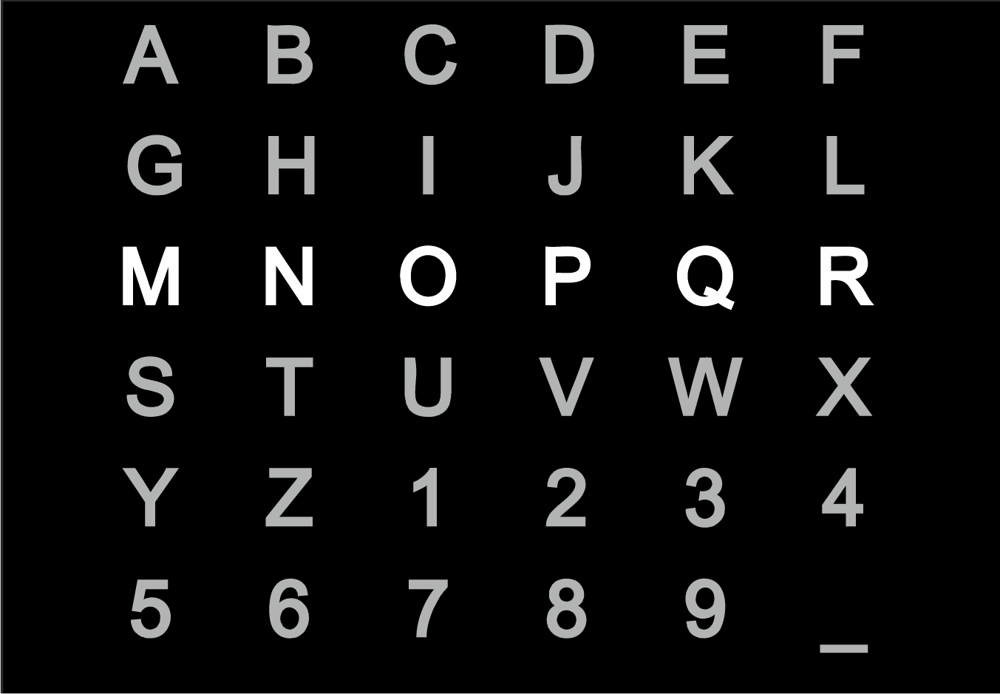
\includegraphics[width=0.3\columnwidth]{\imgpath/speller.png}
  \caption{A speller interface with the third row highlighted.}
  \label{fig:speller}
\end{figure}

Kindermans et al. proposed a method to auto-calibrate the decoder of P300 signals by exploiting multiple source of information \cite{kindermans2012b,kindermans2014integrating}. As for most of the work presented above, they consider transfer learning where a model of previous subjects is used to ``regularizes the subject-specific solution towards the general model''. As it is a spelling task, they also make use of language models as a prior probability on the possible next letter. They also include a dynamic stopping criteria which is a measure of confidence on the next letter allowing the system to stop when it reaches a confidence threshold. Finally, and of more interest for us, they make use of unsupervised learning using an EM algorithm to update the classifier as new data comes in. They exploit the particular fact that among the multiple stimulations only one event out of six encodes a P300 potential in the speller paradigm.

While still requiring to bootstrap the system with several random classifiers as well as a warm-up period, Kindermans et al. have shown their unsupervised learning method coupled with specific properties of the task allows to start interacting with a speller without the need for calibration procedure \cite{Kindermans2012a,kindermans2014true}. This achievement correspond to solving the problem of \emph{learning from unlabeled interaction frame} and is therefore of high interest for our work. We now explain what specific information was used to solve this problem and identify it as being of a very specific nature which differs from all other approaches.

As detailed earlier, the P300 speller problem offers some guarantee on the repartition of ``correct'' and ``incorrect'' P300 events. Only one row and one column should elicit a P300 response. In the case of a 6 rows speller, if each row are systematically scanned the same number of time, only one signal out of 6 will encode a positive P300 signals. And even more informative is the fact that, even if the wrong letter is identified in the end, at least 4 labels out of 6 will be correctly assigned. Indeed, if the correct letter is identified, then the ``correct'' label will be correctly assigned, as well as the five ``incorrect'' labels. If the wrong letter is identified, two labels will be swapped, resulting in two association errors, but still four ``incorrect'' labels will be correctly assigned. In the end, this is quite a lot of information which can offer good guarantees for their EM algorithm to identify properly the ``incorrect'' signal cluster; leaves the second cluster for the ``correct'' signals. As more data are collected, the EM algorithm will be better at identifying the underlying structure of the data and will be able to identify the cluster of ``correct'' from the one of ``incorrect'' given the constraints detailed above. As the process continues, identifying further letter is made easier, and importantly, by going back in the history of interaction, the system can correct those letters that were wrongly identified.

As we will discover in next chapters, our method to do requires to have access to such constraints and guarantees about the task, which makes our work easily generalizable to many types of problems. However, the work of Kindermans et al. already exploits information of a very specific nature to solve the problem of \emph{learning form unlabeled interaction frames}. Contrary to all the other approaches, their information source does not provide a direct knowledge about the task (as a language models do), neither about how to decode the signals themselves (as transfer learning methods do). It rather provides an information emerging for the joint combination of a task and of a signal decoder. That is for the correct task (i.e. the correct letter), only one signal should be classified as ``correct'' and all the others as ``incorrect''. 

\transition

This type of information, that acts neither on the task, neither on the signal decoder, but rather on the combination of both is at the core of the work we will present in forthcoming chapters. As we have seen in section~\ref{chapter:related:language:thomas}, Thomas Cederborg also make us of a similar source of information but reasoning about the consistency of some gestures with respect to different geographical references, e.g. object position. We will summarize those works in next section~\ref{chapter:related:discussion} and highlight the differences and improvements of our method.

\section{Discussion}
\label{chapter:related:discussion}


Yet, to our knowledge, in most of these existing works the interaction protocols have always been pre-programmed (that is the robot knows how to use and understand them innately, e.g. he knows how the teacher expresses ``correct'' or ``incorrect'' feedback), as well as used by the robot learner to strictly identify new (form, meaning) pairs in the sensorimotor flow. The work we present in this thesis shows mechanisms allowing a learner to acquire meaning associated to teaching and guidance signals in the context of social interaction. Furthermore, while in most models of lexicon acquisition no tasks are learned (only word-meaning associations are learned), we show mechanisms allowing the learner to leverage learned word meanings to learn novel tasks from a human.

The methods we present form a basis on which such flexible and adaptive teaching protocols could be learnt.


This discussion section may be worth reading again once the reader has been through chapter~\ref{chapter:lfui}.

We believe our method differs from all the above mentioned approach as we do not start from a random classifier that by definition will produce wrong classification. Our method is also able to produce a confidence measure on its estimation.

In chapter~\ref{chapter:bci}, we will test our algorithm in a BCI application. 

target reaching task

We will use a different type of error related potential signals which will encode a ``correct'' or ``incorrect'' feedback for the agent. Such signals are of similar type that the P300 signals use by Kindermans et al., i.e. they encode a binary event. However they are slower to elicit and are known to be harder to detect \todo{cite smthg}.

we believe our approach is more general

Surprisingly, it is in the BCI domain that the idea of adaptive interface seems to be highly developed. This may be explained by the specific nature of brain signals which are not used to deal with our daily life and therefore could not have any intuition on how to train universal decoder such as has been done for speech recognition. And no a priori on the shape of the signals

Still most the work, while releasing some important aspect of the interaction have access to a direct relation between signals and meaning at some point. To our knowledge, only two works are tackling the same problem as the one presented in this thesis.

 
\cite{cederborg2011imitating}
it is not about a sequetial task. the robot can reproduce a trajectory, do not need planning skills

and

\cite{Kindermans2012a,Kindermans2012b,kindermans2014integrating} not sequetial, use an additonal source of information (specific ratio of each label). Plus they have this eureaka moment, which is the system makes some mistake in the beginning but is abla to recover them after some time. This is manily due to the nature of the task, where to spell on letter only 15 flash for each letter is allowed....

In the following of this thesis we present methods that imporve over the following work, by

sequential task

work without reauiring a specific ratio of signals

based on the coherence between the organization fo signal in the feature space and the labels. explain again the method in few lines

planning

extendtion in continuous states space, continuous task space (finite number of letter, finite number of object), release the need to known the interaction frame, i.e. feedback or guidance, unknown in advance.

proof

However we note that in the core work of this thesis, we will consider optimal teachers and simply model some percentage of teaching mistakes to account for the variability between users.


we will consider teacer are optimal but a bit noisy. this might not be an accruate assumtion givent he work present in sectino about human teaching behavior. However our method is not restricted to the use of optimal teacher, the only requirement is to have access to a human model or several human model as we will se in chapter , among which one is good enough to represent the actual hunan teaching bheavior.

\todo{resue all this in the conlsusion}

generic to any sequential task problem, with any type of interaction frames


We will propose a measure sharing similar properties than their approach in chapter

However we will argue that our method is more generic and can be applied in majority of sequential problems. Indeed for most sequential task, it is impossible to define a sequence of actions that guarantee a specific ratio of meanings in the received signals. 


Our work differs by

In fact kindermans also intialize with a randomly a classifier
that is initialized randomly and updated during usage. Initially, the unsupervised classifier tends to make decoding mistakes, as the classifier might not have seen enough data to build a reliable model.

diff with kindermans: warm up period for them where they make mistakes. We are able to know when we know. + we can apply it to any sequential task, does not requires a specifi ratio + we have planning

